\chapter{Luminosity Calibration at the LHC}

CERN’s mission of understanding the fundamental structure of the universe is heavily reliant on particle accelerators. The effectiveness of the experiments conducted in these machines is closely tied to their luminosity, as detailed in \autoref{sec:luminosity}. 
In this chapter, the van der Meer (vdM) scan methodology used to measure the luminometer's calibration factor is explained first. Subsequently, the corrective procedures applied to optimize the accuracy and precision of this method are discussed. Finally, the challenges associated with extrapolating the results obtained with the vdM method for the rest of the data-taking period are addressed.
\section{Absolute luminosity calibration}
\label{sec:absolute_luminosity_calibration}

As explained in \autoref{subsec:luminosity_calibration}, all luminometers require a specific calibration, $\sigma_{vis}$, to convert their measured rates into an absolute measurement of luminosity. A common limitation in making precise theoretical predictions of Standard Model processes is the uncertainty in the parton distribution functions within the proton \cite{GRAFSTROM201597}. These limitations necessitate methods that do not rely on theoretical assumptions of these distributions. While data-driven methods have been proposed, they introduce correlations between low and high pileup data-taking periods \cite{Salfeld-Nebgen_2018}. A more precise and purely experimental procedure to determine this detector calibration is the van der Meer (vdM) scan methodology.

In order to measure the visible cross section, beam scans are performed, in which the two LHC beams are moved with respect to each other in the transverse ($x-y$) plane in incremental steps. This procedure was pioneered by Simon van der Meer at the Intersecting Storage Rings (ISR) \cite{vanderMeer:296752} and extend by Carlo Rubbia to the case of a collider with bunched beams \cite{Rubbia:1025746}. Instead of measuring the transverse bunch density functions, this method allows for the measurement of the bunch overlap integral from the rates measured at different beam separations. This method has been used by every LHC experiment \cite{TheLHCbcollaboration_2014, ALICE-PUBLIC-2021-001, Maettig:1513982, Sirunyan:2759951}.

\subsection{The van der Meer Scan Methodology}
\label{subsec:the_van_der_meer_scan_methodology}

Recalling \autoref{eq:sbil-machine-params} and \autoref{eq:effective-area}, we can rewrite the SBIL expression for beams separated by $\Delta_x$ in the horizontal plane and $\Delta_y$ in the vertical plane as:

\begin{equation}
    \label{eq:sbil_separating_planes}
    \mathcal{L}_b \left( \Delta_x, \Delta_y \right) = N_1 N_2 f_{rev} \int \rho_1 (x, y) \rho_2 (x + \Delta_x, y + \Delta_y) dx dy
\end{equation}

As shown in \cite{vanderMeer:296752}, when a separation scan is performed in either transverse direction, where $\Delta_x$ and/or $\Delta_y$ is varied in a step-wise manner, the effective width and height of the luminous region can be expressed as:

\begin{equation}
    \begin{aligned}
        \label{eq:effective_width_height_scan}
        W_{eff} = \frac{\int \int \rho_1 (x) \rho_2 (x + \Delta_x) dx d\Delta_x}{\int \rho_1 (x) \rho_2 (x) dx} = \frac{\int \mathcal{L}_b \left( \Delta_x, 0 \right) d\Delta_x}{\mathcal{L}_b \left( 0, 0 \right)} \\
        H_{eff} = \frac{\int \int \rho_1 (y) \rho_2 (y + \Delta_y) dy d\Delta_y}{\int \rho_1 (y) \rho_2 (y) dy} = \frac{\int \mathcal{L}_b \left( 0, \Delta_y \right) d\Delta_y}{\mathcal{L}_b \left( 0, 0 \right)}
    \end{aligned}
\end{equation}

where the beam populations, $N_1$ and $N_2$, and the LHC revolution frequency have been canceled in the second step for both equations.

Assuming Gaussian-distributed bunches, the scan curves $\mathcal{L}_b \left( \Delta_x, 0 \right)$ and $\mathcal{L}_b \left( 0, \Delta_y \right)$ will also be Gaussian. Thus, we arrive at the equality expressed in \autoref{subsec:luminosity_from_machine_parameters}, where $\Sigma_X = \sqrt{2\pi} W_{eff}$ and $\Sigma_Y = \sqrt{2\pi} H_{eff}$, thereby proving the equivalence of the method. However, as mentioned at the beginning of this section, no assumptions are made about the nature of the particle bunch distribution, which means the scan curves are not guaranteed to be Gaussian.

Frequently, these curves are not well described by simple Gaussians. In this analysis, we fit these curves with Double Gaussian (DG) functions of the form:

\begin{equation}
    f_{\text{DG}}(\chi) = 
    \frac{r_{\chi}}{\sqrt{2\pi}} 
    \left[ 
        \frac{\epsilon_{\chi}}{\sigma_{1_{\chi}}} \text{exp} \left( -\frac{\left( \Delta_{\chi} - \mu_{\chi} \right)^2}{2\sigma^2_{1_{\chi}}} \right) +
        \frac{1 - \epsilon_{\chi}}{\sigma_{2_{\chi}}} \text{exp} \left( -\frac{\left( \Delta_{\chi} - \mu_{\chi} \right)^2}{2\sigma^2_{2_{\chi}}} \right)
    \right]
    \label{eq:double_gaussian_model}
\end{equation}

where $\chi \in \{X, Y\}$ denotes the scanning plane, $\Delta_{\chi}$ is the nominal beam separation, $r_{\chi}$ and $\mu_{\chi}$ are the peak and peak position of the DG and $\sigma_{1_{\chi}}$, $\sigma_{2_{\chi}}$ are the widths of the two individual Gaussians. The two Gaussians are weighted by $\epsilon_{\chi}$ and $1 - \epsilon_{\chi}$, respectively, and $\Sigma_{X}$ and $\Sigma_{Y}$ are related to the individual beam widths by: 

\begin{equation}
    \Sigma_{\chi} = \frac{\sigma_{1_{\chi}}\sigma_{2_{\chi}}}{\epsilon_{\chi}\sigma_{2_{\chi}} + \left( 1 - \epsilon_{\chi}\right) \sigma_{1_{\chi}}}
\end{equation}

The visible cross section, $\sigma_{vis}$, can also be expressed as a function of the fit parameters as:

\begin{equation}
    \sigma_{\mathrm{vis}} =  \frac{2\pi \Sigma_{X} \Sigma_{Y} R_{peak}}{N_1 N_2 f_{rev}}
    \label{eq:calibration_from_fit_parameters}
\end{equation}

where $R_{peak}$ is taken as the arithmetic mean of the peak values, $r_X$ and $r_Y$, of both scan curves. This fit procedure is applied for every bunch crossing. Since the visible cross section results heavily dependent on how well the fit converges we only apply this method on the luminometers which have per-bunch granularity.

\autoref{fig:vdm_scan_steps} illustrates the beam separations during two vdM scans, one in each transverse direction.

\begin{figure}[!htb]
	\centering
	\includegraphics[width=\textwidth]{images/assets/vdm_scan_steps.png}
	\caption[Example vdM scan sequence positions]{Nominal LHC beam positions displaying the van der Meer scan sequence first in $x$-axis and then in $y$-axis (from \textit{Ref.} \cite{Saariokari:2826125}).}
	\label{fig:vdm_scan_steps}
\end{figure}

\subsection{Experimental Conditions and Corrective Procedures}
\label{sec:experiment_conditions_and_corrective_procedures}

A vdM scan is conducted under experimental conditions that allow for the measurement of the visible cross section to the highest precision. These conditions include smaller beam intensities, which minimize the effect of BIB and reduce non-linearity effects, and well-separated bunches, which minimize afterglow effects \cite{GRAFSTROM201597}. In addition to these optimized experimental conditions, a series of offline corrections are performed to ensure the required level of precision. These corrections include:

\begin{itemize}
    \item \textbf{Background estimation:} Background signals, whether beam-induced, from detector noise, or machine-induced, are typically present in the raw recorded rates. These additional contributions are removed.
    \item \textbf{Beam current measurement:} Various systems measure and monitor the beam conditions throughout the entire fill to enable offline corrections, such as the removal of spurious charges.
    \item \textbf{Beam-beam effects:} The electromagnetic interaction between the two LHC beams causes disturbances in the nominal beam separation and shapes, affecting the calibration measurement \cite{Babaev2024}. These effects are accounted for and corrected in the analysis.
    \item \textbf{Orbit drift:} During the vdM fill, the nominal position of the LHC beams may shift. These shifts are measured by Beam Position Monitors (BPM), which provide information to correct the nominal beam separations.
    \item \textbf{Length scale calibration:} The operational displacement of the LHC beams is achieved using a pair of steering dipoles located on either side of the IP. These displacements come with associated uncertainties due to effects such as magnet hysteresis or lattice imperfections \cite{Persson:2750277}. These effects are taken into account.
    \item \textbf{XY factorization:} The vdM method assumes that the transverse particle distributions are independent in each transverse direction and therefore factorizable. If this assumption is not true, the calculated value for \(A_{eff}\) will be biased. Studies are conducted to understand the magnitude of this bias and correct it.
\end{itemize}

A more detailed explanation of these corrections, as well as their impact on the measured calibration, will be provided in \autoref{ch:2023_luminosity_calibration}.

\subsection{Extrapolation of vdM Calibration}
\label{subsec:extrapolation_of_vdM_calibration}

The experimental conditions in which a vdM fill is performed, as well as all the extra corrections applied to the collected data, ensure a visible cross section measurement with high precision and accuracy. However, the optimal experimental conditions for probing the Standard Model, known as ``physics conditions", introduce several effects that impact the calibration of the luminometers. Therefore, it is necessary to extrapolate the results obtained during a vdM fill to correctly calibrate the luminosity measured under physics conditions.

Physics conditions are tailored to obtaining the largest amount of data possible. This includes higher bunch populations compared to vdM fills and more colliding bunches, all of which increase the number of colliding particles. These conditions bring about two classes of effects on our luminometers:

\begin{itemize}
    \item \textbf{Efficiency effects:} Prolonged exposure to ionizing radiation from highly-energetic interactions deteriorates the luminometers, making them less efficient. These effects result in a gradual decrease in the reported luminosity throughout the data-taking period.
    \item \textbf{Non-linearity effects:} Varying experimental conditions can affect the reported luminosity of our detectors, as mentioned in \autoref{subsec:luminosity_detectors}. While some of these effects have their own corrective procedures, such as out-of-time pileup \cite{Sirunyan:2759951}, others are corrected empirically.
\end{itemize}

To account for these two classes of effects, the measured luminosity undergoes a final correction described by \autoref{eq:luminosity_integration}.

\begin{equation}
    \centering
    \mathcal{L} = \frac{f_{rev} \cdot \mu}{\sigma_{vis} \cdot \epsilon} - \alpha \left( \frac{f_{rev} \cdot \mu}{\sigma_{vis} \cdot \epsilon} \right)^{2}
    \label{eq:luminosity_integration}
\end{equation}

Two new parameters have been introduced. \(\epsilon\) is the parameter that corrects for losses in detector efficiency throughout the data-taking period. To obtain these factors, mini vdM-like scans, called emittance scans (em), are performed. These scans are used to measure the visible cross section using the same vdM method, allowing for the analysis of the evolution of this quantity over the data-taking period. A figure of merit (FOM) is then calculated as:

\begin{equation}
    \centering
    \text{FOM} = \frac{\sigma^{\text{vdM}}_{vis}}{\sigma^{\text{emit}}_{vis}}
    \label{eq:figure_of_merit}
\end{equation}

where \(\sigma^{\text{vdM}}_{vis}\) is the visible cross section measured under vdM conditions, and \(\sigma^{\text{emit}}_{vis}\) is the visible cross section measured during emittance scans under physics conditions. These FOM values are calculated for every emittance scan throughout the data-taking period and used to correct for variations in each luminometer's efficiency.

The second new parameter, \(\alpha\), corrects for any non-linearity in the luminometers and is derived empirically. Non-linearity is defined as any non-linear response to changes in experimental conditions. \autoref{fig:non_linearity_diagram} illustrates the response of a theoretical linear detector, a detector with positive non-linearity, and a detector with negative non-linearity.

\begin{figure}[!htb]
    \centering
    \makebox[\textwidth]{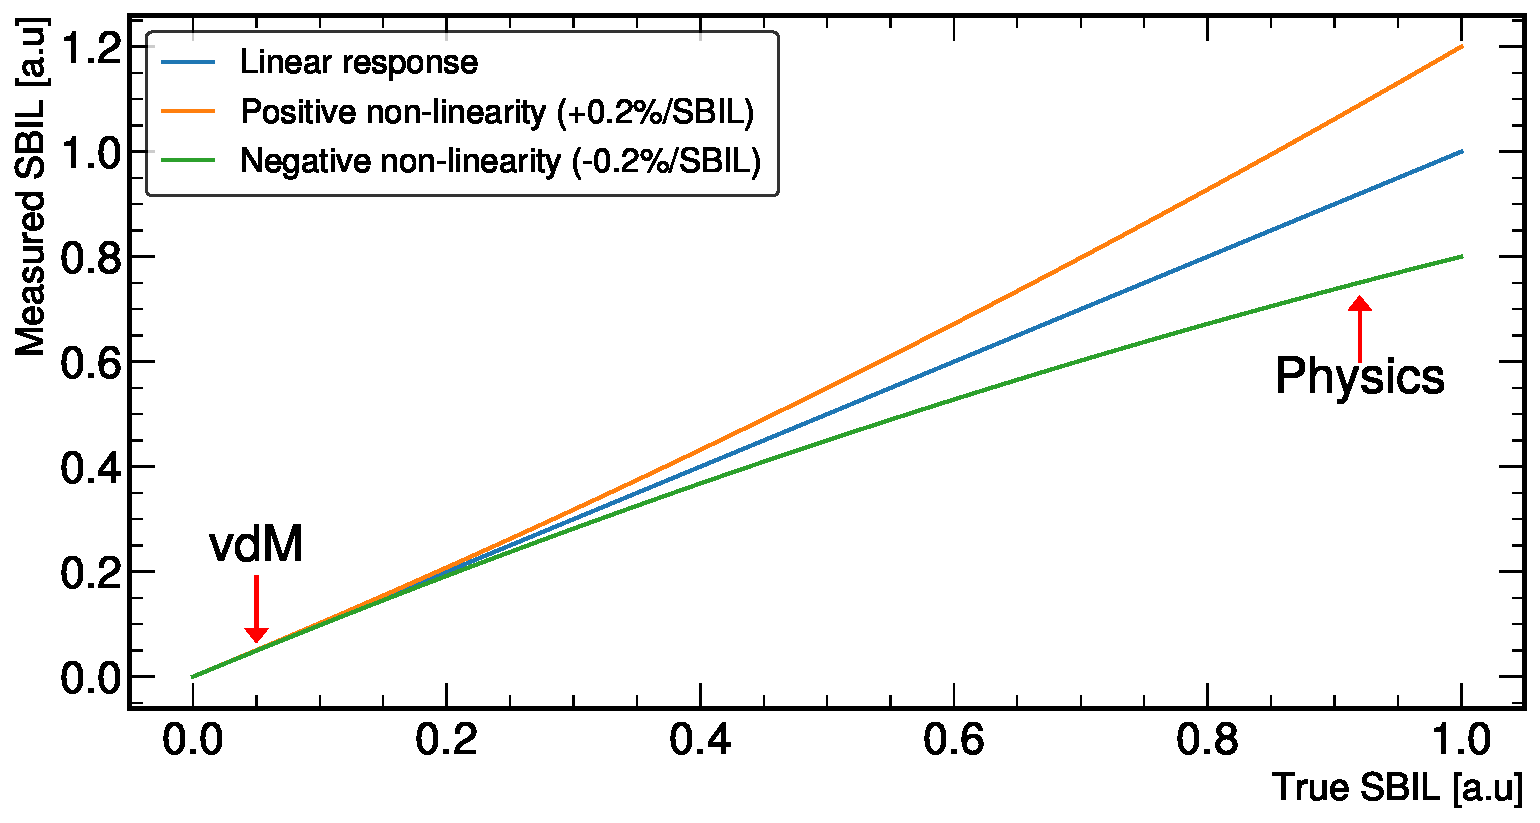
\includegraphics[width=0.7\paperwidth]{images/assets/non_linearity_diagram.pdf}}
    \caption[Non-linearity effects on SBIL]{Illustration of non-linearity effects on measured SBIL as a function of the true SBIL. The two marked regions illustrate the effects of extrapolating from vdM to physics conditions.}
    \label{fig:non_linearity_diagram}
\end{figure}

The reasons for a detector to have a positive or negative non-linear response vary:

\begin{itemize}
    \item PLT has consistently shown signs of positive non-linearity, mainly due to the increased probability of ``accidental" triple coincidences at higher pileup due to background tracks, leading to over counting.
    \item HFOC suffers from the ``zero starvation" effect, as explained in \autoref{subsec:zero-counting}, leading to an underestimation of the measured rates, categorized as negative non-linearity.
\end{itemize}

Correcting for non-linearity is challenging due to the lack of a perfectly linear reference detector. Instead, a reference detector, assumed to be linear, is used. In this method, a linear fit is performed on the ratio between a luminometer and this reference detector as a function of SBIL. 

The slope extracted from the fit is then used as the value of \(\alpha\) in \autoref{eq:luminosity_integration}. Unlike the efficiency corrections (\(\epsilon\)), the non-linearity corrections are done at the expense of introducing some degree of correlation between the corrected detector and the reference. To keep the luminometers as independent as possible, the slopes are extracted for only a few fills with a high SBIL range throughout the year.

The specialized vdM conditions, along with the series of corrections applied to the vdM data and the extrapolation to physics conditions, all contribute to the significant challenge of accurately measuring luminosity at hadron colliders like the LHC.

\subsection{Additional Scans}

In addition to the vdM scan, other types of scans are performed during the vdM fill to provide specific insights into the various experimental conditions:

\begin{itemize}
    \item \textbf{Super Separation scans (ss):} These scans involve maximally separating the beams in the LHC, allowing for an accurate measurement of the background for each luminometer.
    \item \textbf{Beam Imaging scans (im):} In these scans, one beam is kept fixed in its nominal head-on position while the other beam is scanned. These scans are used for the beam-imaging method \cite{Klute_2017}, which is employed in XY factorization analysis. A visible cross section is also extracted from these scans, similar to vdM scans.
    \item \textbf{Diagonal scans (diag):} These are vdM scans performed at distinct angles, such as +45º/-45º, +30º/-60º, and +60º/-30º. They allow the fitting to occur over different regions of the beam overlap and are used in XY factorization studies.
    \item \textbf{Offset scans (off):} These scans have the same motion as vdM scans, but one of the beams is not in the nominal head-on position. They are used in beam shape studies to determine the XY factorization bias.
    \item \textbf{Variable/Constant length scale scans (vls, cls):} These scans involve moving the beams together at constant or variable separation and are used to calibrate the distance by which the steering magnets displace the beams.
\end{itemize}

Each scan is separately recorded and analyzed offline. After thorough analysis, the corrective procedures determined from each of these special scans are applied to the vdM scan analysis to correct the extracted detector calibration. In principle, these corrections affect every luminometer in a similar fashion.
